% !TEX root = ../exercises.tex
\section{Primary Positrons from Galactic Pulsars}

Galactic pulsars, particularly those associated with bow shocks, are believed to be the main contributors to cosmic-ray positrons. 

The luminosity of bow-shock pulsars, in terms of pairs, is given as a function of time (\(t\)):
%
\[\mathcal{L}_{\text{bs}}(t) = \frac{1}{2} I \Omega_0^2 \frac{1}{\tau_0} \frac{1}{\left(1+\frac{t}{\tau_0}\right)^2}\]
%
where $I = \frac{2}{5} M R^2$ is the moment of inertia, $\Omega_0 = \frac{2\pi}{P_0}$ is the angular frequency, and $\tau_0$ is the spin-down age.

The cosmic-ray positron flux at \(E = 100\) GeV is measured to be (see plot):
%
\[E^2 \Phi \approx 0.15 \, \text{GeV m}^{-2} \text{s}^{-1} \text{sr}^{-1}\]
%
\begin{center}
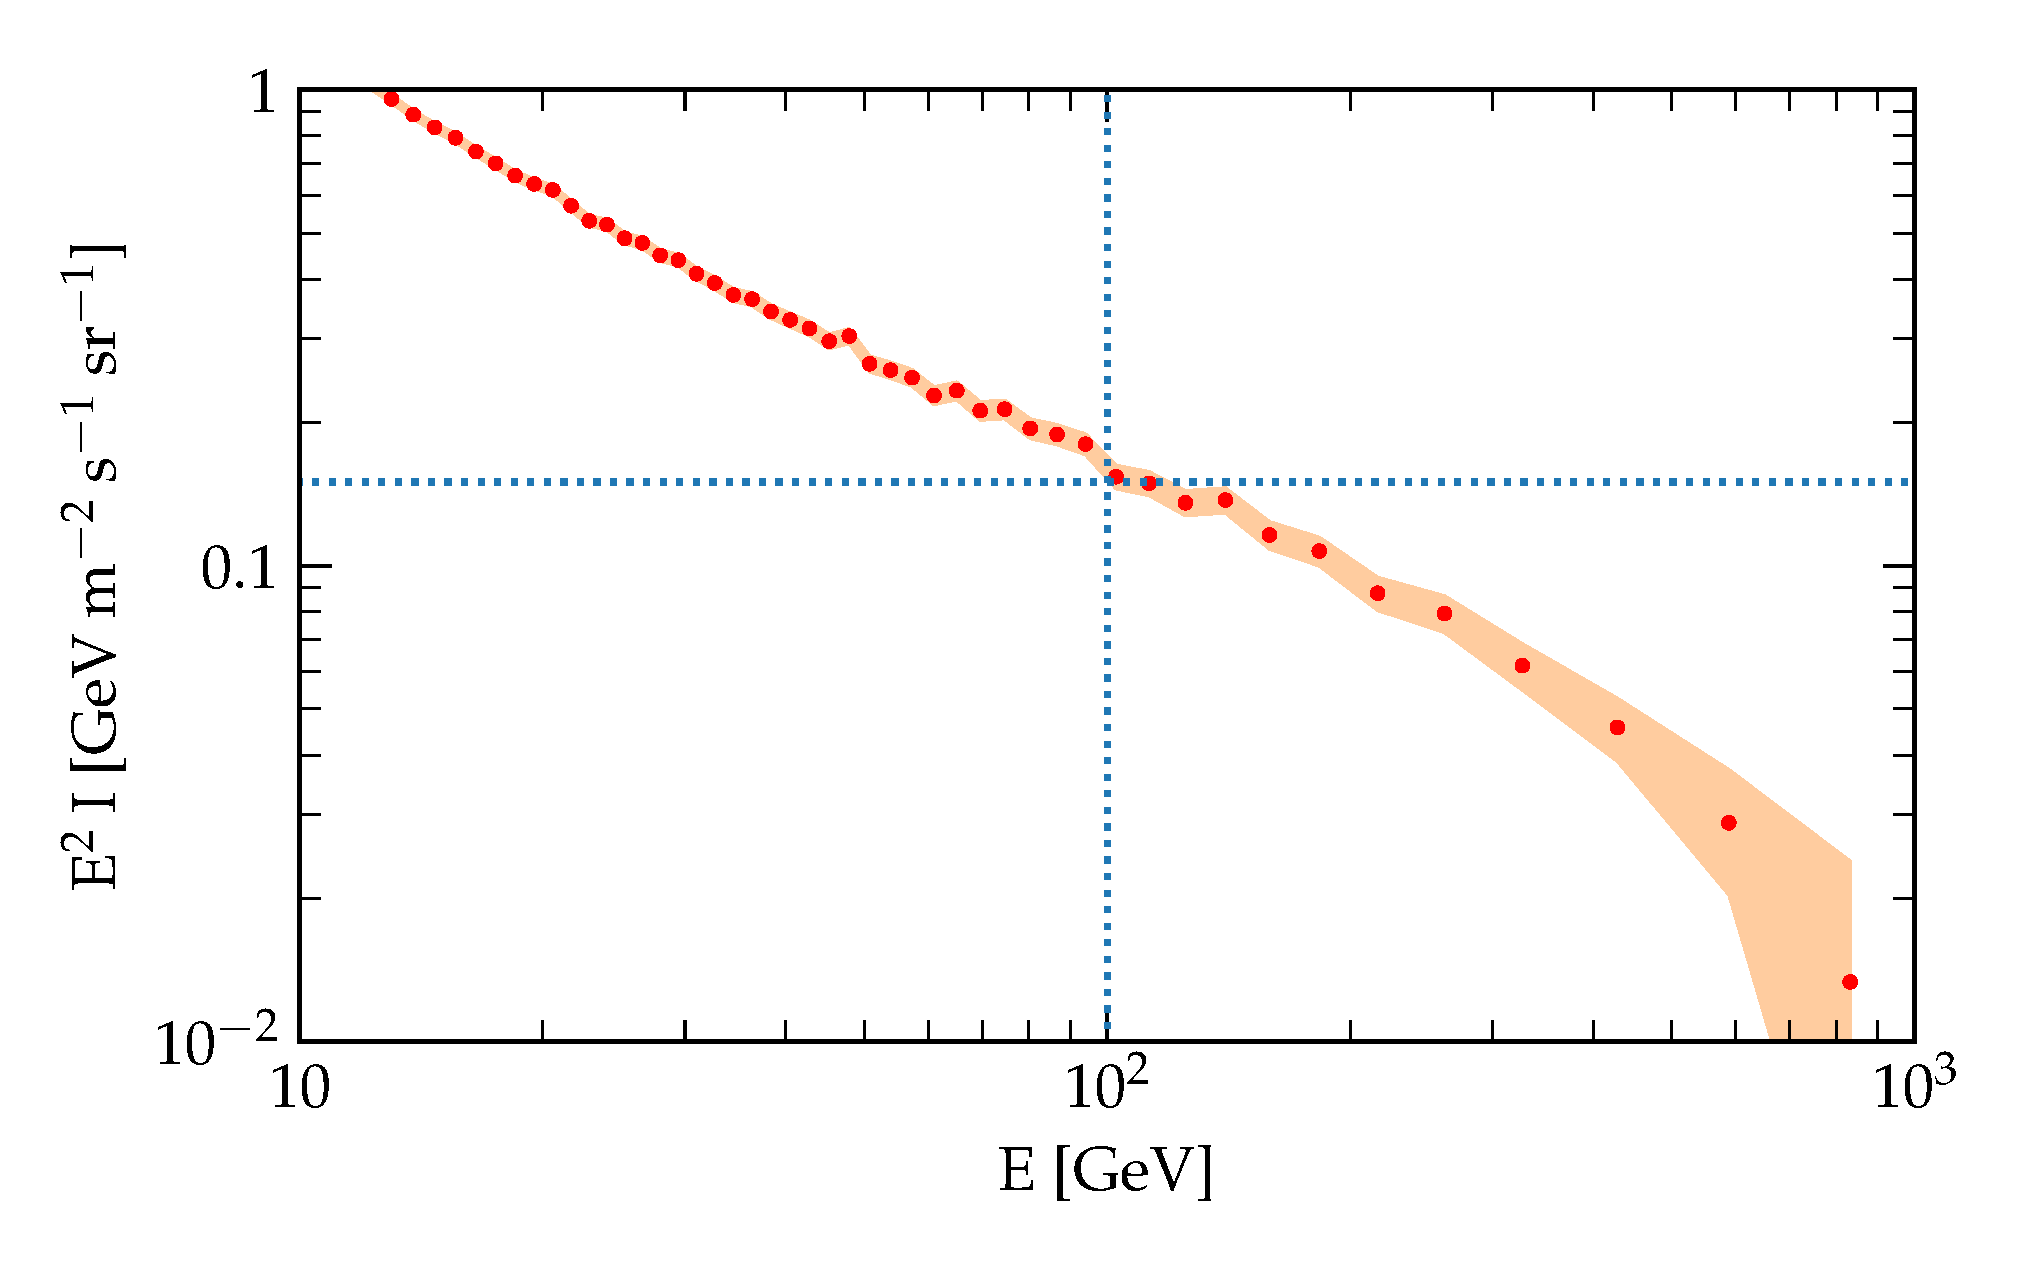
\includegraphics[scale=0.25]{figures/ex_positrons.pdf}
\end{center}

\begin{itemize}
%%\item Calculate the positron energy density corresponding to the observed flux. 
\item Compute the total energy in the form of positrons released by the pulsars \( E_{\rm bs}\) for \(t \gg \tau_0\), assuming \( P_0 = 0.1\) s\(^{-1}\), $M = 1.4 \, M_\odot$, $R = 10$ km.
\item With a given rate of \(\mathcal{R} \sim 2/\)century and an efficiency \(\xi < 1\), estimate the local energy density of positrons at the same energy $E = 100$~GeV. Assume a diffusion coefficient \(D(E) = 3 \times 10^{28} (E/\text{GeV})^{1/2}\) cm\(^2\)/s, halo size \( H = 5 \)~kpc, and consider energy losses due to Inverse Compton scattering on the CMB and synchrotron radiation in a \(3 \mu\)G magnetic field.
The spectrum released by the pulsars is assumed to be $\propto E^{-1}$ up to a maximum energy of $E = 100$ GeV.

\item Derive the value of \(\xi\) by comparison with the measured value.

\end{itemize}

